\section{Results}\label{sec:results}
\subsection{Inference Latency Testing}\label{subsec:inference-latency-testing}
\subsubsection{Methodology}
Unfortunately, it is not currently possible to test the inference latency performance of most neural networks architectures tested directly on the Arduino Nano 33 BLE\@.
As mentioned in section~\ref{sec:model-implementation}, the TensorFlow library is used to train the neural networks, while TensorFlow Lite for Microcontrollers is used run inference on them.
However, the Arduino implementation of TensorFlow Lite for Microcontrollers does not currently have support for recurrent neural networks, which are also needed for all other architectures tested excluding transformer encoders.
While it is possible to use RNNs with the most recent version of TensorFlow Lite for Microcontrollers (version 2.9), the library's Arduino implementation is a few versions behind (currently version 2.4), and is outdated enough that it is missing certain tensor operations necessary for running RNNs and their derivatives.

Therefore, a different method was used to estimate the inference latency of RNNs on Arduino.
Since regular artificial neural networks are compatible with TensorFlow Lite for Microcontrollers version 2.4, several configurations of these with varying neuron and densely connected layer counts were trained and deployed on the Arduino Nano 33 BLE\@.
These configurations are listed in table~\ref{tab:ann_configs}, formatted as (number of densely connected layers layers/number of neurons per layer).
Each configuration also includes a final densely connected layer of 10 neurons for output.
Since ANNs require 1D input data, a dummy data instance was taken from the dataset and flattened into a single array of 300 values (3 photodiodes $\times$ 100 samples).
This dummy data instance was then used as input to the networks so that their latencies could be measured.
The inference times of these generic networks on the Arduino Nano 33 BLEs were compared to their TensorFlow Lite file (.tflite extension) sizes, to see if file size could be used to predict inference latency.

\begin{table}[]
    \centering
    \captionsetup{justification=centering}
    \begin{tabular}{lll}
        Configuration & File Size (MB) & Latency (ms) \\
        \hline
        (1/128)       & 42             & 103.9        \\
        (1/256)       & 81             & 179.6        \\
        (1/512)       & 160            & 333.0        \\
        (2/64)        & 27             & 74.7         \\
        (2/128)       & 59             & 134.5        \\
        (2/256)       & 147            & 293.7        \\
        (4/32)        & 17             & 55.4         \\
        (4/64)        & 59             & 92.3         \\
        (4/128)       & 93             & 195.0
    \end{tabular}
    \caption{Table comparing the file sizes and inference latencies of various TensorFlow Lite artificial neural networks.}
    \label{tab:ann_configs}
\end{table}

\subsubsection{Results}
Figure~\ref{fig:latency_results}\@ illustrates that a neural network's inference latency can indeed be estimated using the function $y = 1.89x + 23.6$, where $x$ is the model file size in kilobytes and $y$ is the model's expected inference latency in milliseconds.

\begin{figure}[h]
    \centering
    \captionsetup{justification=centering}
    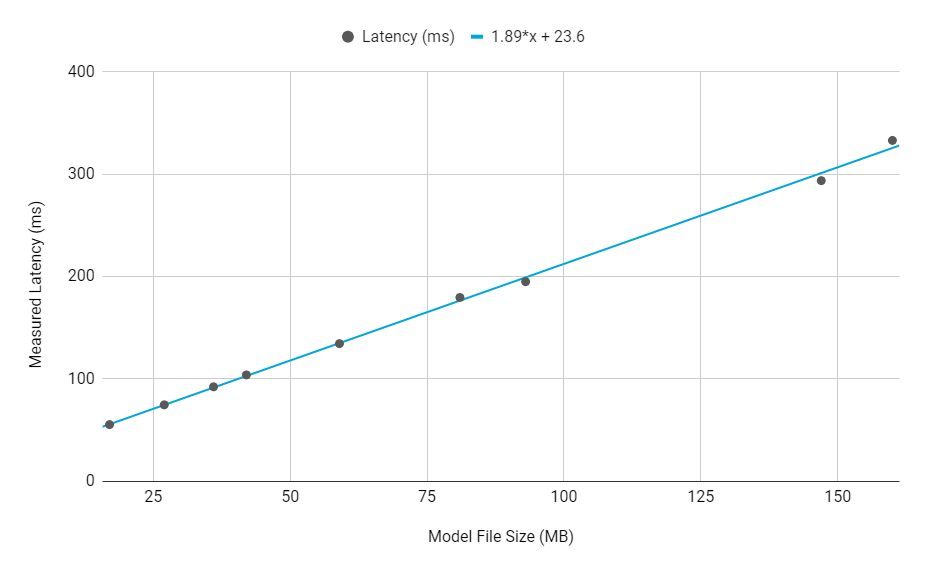
\includegraphics[width=\linewidth]{figures/latency_results}
    \caption{Graph showing the relationship between file size and inference latency for various TensorFlow Lite artificial neural networks.}
    \label{fig:latency_results}
\end{figure}

However, it is worth noting that the largest model for which latency was tested, with a 160KB file size, only produced a latency of 333 milliseconds despite using 97\% of the available RAM on the Arduino Nano 33 BLE (this memory usage includes the boilerplate code needed for loading and running the model).
A latency of 333ms is similar to human reaction time (CITATION NEEDED) and can therefore be considered real-time for the purpose of gesture recognition.
Therefore, inference latency is not much of a concern, though it is important that all models tested in this study do not exceed a file size of \~160KB, so that they could be run on the Arduino in the future.

\subsection{Accuracy Testing}\label{subsec:accuracy-testing}
\subsubsection{Methodology}
To ensure that the measured validation accuracy was representative across all neural network architectures tested, four distinct measures were put in place:
\begin{enumerate}
    \item A dropout layer with $p=0.5$ was added before the output layer for each architecture to reduce overfitting~\cite{JMLR:v15:srivastava14a}.
    \item K-fold cross-validation~\cite{inbook} was used with $k=5$, as validation accuracy can be skewed based on how the test and validation sets are split.
    \item Each neural network was trained until the value of the validation function no longer improved for 100 consecutive epochs, mitigating the variation in training time caused by randomizing initial neuron weights as well as differences in architecture.
    \item Data instances for each participant in the dataset were shuffled randomly, as ordered data can cause slow training times and poor performance.
    However, the order of participants was not shuffled to ensure that gestures in the training data were recorded by different participants to gestures in the validation data, making validation more representative of a real-world scenario.
\end{enumerate}

\section{Accuracy Testing}\label{subsec:accuracy-testing-results}
\subsubsection{RNN}

\subsubsection{LSTM}

\subsubsection{GRU}

\subsubsection{CNN+LSTM}

\subsubsection{Transformer Encoder}
